%Este trabalho está licenciado sob a Licença Creative Commons Atribuição-CompartilhaIgual 3.0 Não Adaptada. Para ver uma cópia desta licença, visite https://creativecommons.org/licenses/by-sa/3.0/ ou envie uma carta para Creative Commons, PO Box 1866, Mountain View, CA 94042, USA.

%%%%%%%%%%%%%%%%%%%%%%%%%%%%%%%%%%%%%%%%%%
% ATENÇÃO
%
% POR SEGURANÇA, NÃO EDITE ESTE ARQUIVO
%
%%%%%%%%%%%%%%%%%%%%%%%%%%%%%%%%%%%%%%%%%

\documentclass[12pt]{book}

\input preambulo.tex


\begin{document}

\frontmatter

%titlepage
\title{Cálculo}
\date{\today\vspace{1cm}\\\small{Veja página do projeto em:\\
\url{https://www.ufrgs.br/reamat}}}

\maketitle
%\makeindex





% v.4 copyright page
\newpage

\par Este trabalho está licenciado sob a Licença Creative Commons Atribuição-CompartilhaIgual 3.0 Não Adaptada. Para ver uma cópia desta licença, visite http://creativecommons.org/licenses/by-sa/3.0/ ou envie uma carta para Creative Commons, PO Box 1866, Mountain View, CA 94042, USA.
.\index{licença}



\tableofcontents
\listoffigures

\listoftables

\cleardoublepage
\chapter*{Introdução}

Este livro é de Cálculo. Para um livro de análise, veja \cite{Rudin}.
%%
% Start the main matter (normal chapters)
%\mainmatter


%%%%%%%%%%%%%%%%%%%%%%%%%%%%%%%%%%%%%%%%
%%%%%%%%%%      Parte 1       %%%%%%%%%%
%%%%%%%%%%%%%%%%%%%%%%%%%%%%%%%%%%%%%%%%
\part{Cálculo de uma variável}

\chapter{Limites}
O limite é ... 
\chapter{Derivadas}

\chapter{Estudo das funções contínuas e diferenciáveis}

\chapter{Aplicações das derivadas}

\chapter{Integração}

\chapter{Técnicas de integração}

\chapter{Aplicações da integração}

\chapter{Sequências e séries} 

%%%%%%%%%%%%%%%%%%%%%%%%%%%%%%%%%%%%%%%%
%%%%%%%%%%      Parte 2       %%%%%%%%%%
%%%%%%%%%%%%%%%%%%%%%%%%%%%%%%%%%%%%%%%%

\part{Cálculo de várias variáveis}

\chapter{Curvas no plano}
aa
%Este trabalho está licenciado sob a Licença Creative Commons Atribuição-CompartilhaIgual 3.0 Não Adaptada. Para ver uma cópia desta licença, visite http://creativecommons.org/licenses/by-sa/3.0/ ou envie uma carta para Creative Commons, PO Box 1866, Mountain View, CA 94042, USA.

\chapter{Álgebra vetorial}
O objetivo deste capítulo é revisar conceitos básicos do cálculo e da álgebra linear necessários ao entendimento do cálculo vetorial.    

\section{Vetores e escalares}
Na álgebra linear, vetores\index{vetor} são definidos de forma abstrata como os elementos de um espaço vetorial\index{espaço vetorial}. Os vetores são, então, os elementos de um conjunto em que estão definidas duas operações: a soma de vetores e o produto de vetores por escalares obedecendo as propriedades (\ref{defel}). Um escalar\index{escalar} é um número real ou complexo. Quando o corpo de escalares é o conjunto dos números reais, então dizemos que o espaço vetorial é real. Quando o corpo de escalares é o conjunto dos números complexos, dizemos que o espaço vetorial é complexo. Usaremos uma letra latina com uma seta para denotar vetores ($\vct{u}$, $\vct{v}$ e $\vct{w}$).  Para que um espaço vetorial esteja bem definido, as seguinte propriedades devem ser satisfeitas:

\begin{obs} O vetor nulo $\vct{0}$ e escalar nulo $0$ são entidades matemáticas distintas e não devem ser confundidas.\end{obs}
\begin{subequations}\label{defel}
\begin{align}
\vct{u}+\vct{v}&=\vct{v}+\vct{u},&\mytext{(Comutatividade da soma)}\label{defelcom}\\
\vct{u}+\left(\vct{v}+\vct{w}\right)&=\left(\vct{v}+\vct{u}\right)+\vct{w},&\mytext{(Associatividade da soma)}\label{defelass}\\
\left(\alpha+\beta\right) \vct{u}&=\alpha\vct{u}+\beta\vct{v},&\mytext{(Distributividade da multiplicação)}\label{defeldist1}\\
\alpha \left(\vct{u}+\vct{v}\right)&= \alpha \vct{u}+\alpha\vct{v},&\mytext{(Distributividade da soma)}\label{defeldist2}\\
\alpha \left(\beta\vct{u}\right)&=\left(\alpha\beta\right)\vct{u},\label{defeldist3}\\
\vct{0}+\vct{v}&=\vct{v}, &\mytext{(Existência do vetor nulo)}\label{defelnulo}\\
0\vct{v}&=\vct{0},\label{defelnulo2}\\
1\vct{v}&=\vct{v}.&\mytext{(Elemento neutro)}\label{defelneutro}
\end{align}
\end{subequations}

Observamos que a propriedade associativa dada por (\ref{defelass}) permite que se escreve a soma de três vetores $\vct{u}+\vct{v}+\vct{w}$ sem risco de ambiguidade. A propriedade (\ref{defeldist3}) é algumas vez chamada de associatividade, no entanto, é cauteloso observar que ela não estabelece a associatividade de uma operação, já que o produto de escalares é uma operação distinta do produto de um escalar por um vetor. A propriedade (\ref{defelnulo}) garante a existência de um vetor nulo que funciona com um elemento neutro da soma vetorial. 

A subtração de dois vetores é definida por
\begin{equation}\label{delsub}
\vct{u}-\vct{v}=\vct{u}+ (-1) \vct{v}.
\end{equation}
O vetor $(-1) \vct{v}$ é também denotado por $-\vct{v}$ e tem a seguinte propriedade:
\begin{equation}\label{delinvad}
\vct{v}+(-\vct{v})=\vct{v}+(-1) \vct{v} = (1-1)\vct{v}=0\vct{v}=\vct{0}.
\end{equation}

Um conjunto de vetores $\{\vct{v}_1, \vct{v}_2,\ldots, \vct{v}_n\}$ é dito linearmente dependente (LD), se existem escalares $\{\alpha_1,\alpha_2,\ldots, \alpha_n\}$ com pelo menos um $\alpha_i\neq 0$ tal que
$$\sum_{i=1}^n\alpha_i \vct{v}_i=\vct{0}$$ 
Analogamente, um conjunto de vetores $\{\vct{v}_1, \vct{v}_2,\ldots, \vct{v}_n\}$ é dito linearmente independente (LI) se a identidade 
$$\sum_{i=1}^n\alpha_i \vct{v}_i=\vct{0}$$ 
implica necessariamente que
$$\alpha_1=\alpha_2=\ldots=\alpha_n=0.$$

Um conjunto de vetores LI $B=\{\vct{e}_1, \vct{e}_2,\ldots, \vct{e}_n\}$ é dito uma base para um espaço vetorial $V$ se todo vetor $\vct{v}\in V$ pode ser escrito como uma combinação linear dos vetores de $B$:
$$\vct{v}=\sum_{i=1}^n \alpha_i \vct{e}_i.$$ 

Um espaço vetorial é dito de dimensão finita se admite uma base composta por um número finito de elementos.

\begin{teo}\label{teo_dim} Seja $V$ um espaço vetorial e $E=\{\vct{e}_1, \vct{e}_2,\ldots, \vct{e}_n\}$ e $F=\{\vct{f}_1, \vct{f}_2,\ldots, \vct{f}_m\}$ duas bases de $V$. Então $n=m$. Em outras palavras, todas as bases de espaço linear de dimensão finita têm o mesmo número de elementos.
 \end{teo}

A importância deste teorema reside no fato de permitir a definição de dimensão de um espaço vetorial como sendo o número de elementos de uma base. Esta definição está bem posta, uma vez que este número independe da escolha de base.

Outro conceito importante em espaços reais de dimensão finita é o de orientação de uma base\index{orientação}. O leitor já deve estar familiarizado com o conceito de orientação dextrogira e levogira\index{dextrogira}\index{levogira}\index{regra da mão direita}\index{regra da mão esquerda} (regra da mão direita e esquerda) no espaço tridimensional. No entanto este conceito pode ser estendido de forma natural para espaços reais de n-dimensões. Formalmente falando duas bases $B_1$ e $B_2$ têm a mesma orientação se o determinante da transformação linear que liga $B_1$ a $B_2$ é positivo.    

O espaço vetorial real de $n$ dimensões é denotado $\mathbb{R}^n$. 

\section{O espaço euclidiano tridimensional}
Nossa principal preocupação neste curso é com o espaço euclidiano de três dimensões, dada sua importância para descrição do espaço na física clássica.  
 
O leitor já tem familiaridade com o sistema de coordenadas cartesianas\index{Sistema de coordenadas cartesianas} ($xyz$) para representar um ponto no espaço euclidiano tridimensional. Neste sistema, também chamado referencial cartesiano, cada ponto é representado por um conjunto de três coordenadas $x$, $y$ e $z$. Observamos que existem duas maneiras distintas de orientar tal sistema: usando a regra da mão direita e a regra da mão esquerda, que recebem o nome de dextrogira e levogira, respectivamente. Neste texto, daremos preferência pela orientação dextrogira, que convencionaremos como padrão. Uma vez escolhido um sistema dextrogiro como base,  um trio de vetores linearmente independentes $\vct{u}$, $\vct{v}$ e  $\vct{w}$ é dito dextrogiro\index{dextrogira}\index{levogira}\index{regra da mão direita}\index{regra da mão esquerda} se o determinante 
\begin{equation}\label{defdextro}
\det\left(\vct{u};\vct{v};\vct{w}\right)
\end{equation}   
é positivo. Reciprocamente, o trio  $\vct{u}$, $\vct{v}$ e  $\vct{w}$ é dito levogiro se o determinando for negativo. Veja mais detalhes no exemplo (\ref{probdextro}).

\begin{figure}\begin{center}
 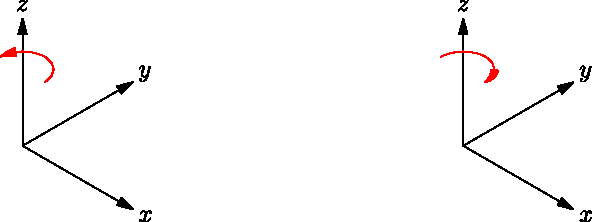
\includegraphics{./cap_algvet/pics/eixos_levo_destro}
      \caption{À esquerda, um sistema levogiro (regra da mão esquerda). À direita, sistema dextrogiro (regra da mão direita).}
      \label{fig:marginfig}
      %\setfloatalignment{b}% forces caption to be bottom-aligned
  \end{center}
  \end{figure}
 
 Um vetor é representado neste sistema como um trio de números reais, denominados componentes do vetor $\vct{v}$ e denotados por: 
\begin{equation}\label{defeucv}\vct{v}=\left<v_1,v_2,v_3\right>.\end{equation}
  
É natural neste momento definir os vetores $\vct{i}$, $\vct{j}$ e $\vct{k}$ como
\begin{equation}\label{defijk}
\begin{array}{rcl}
\vct{i}&=&\left<1,0,0\right>\\
\vct{j}&=&\left<0,1,0\right>\\
\vct{k}&=&\left<0,0,1\right>
\end{array}
\end{equation}
de forma que a expressão (\ref{defeucv}) pode ser escrita como
\begin{equation}\label{repijk}\vct{v}=v_1  \vct{i}+v_2  \vct{j}+v_3 \vct{k}.\end{equation}
O vetor nulo é definido como vetor cujas três coordenadas são nulas:
\begin{equation}\label{defnulo}\vct{0}=0 ~\! \vct{i}+0~\!  \vct{j}+0~\!  \vct{k}= ~\!\left<0,0,0\right>.\end{equation}
A soma de dois vetores é dada pela soma componente a componente, ou seja, se $\vct{u}=u_1  \vct{i}+u_2\vct{j}+u_3 \vct{k}$ e $\vct{v}=v_1\vct{i}+v_2\vct{j}+v_3 \vct{k}$, então
\begin{equation}\label{defsoma}\vct{u}+\vct{v}= \left(u_1+v_1\right) \vct{i}+\left(u_2+v_2\right) \vct{j}+\left(u_3+v_3\right) \vct{k}.\end{equation}
O produto de um vetor por um escalar é definido como a multiplicação componente a componente pelo escalar, ou seja, se $\vct{u}=u_1~\!  \vct{i}+u_2~\!  \vct{j}+u_3 ~\! \vct{k}$, então
\begin{equation}\label{defprod}\alpha\vct{u}=(\alpha u_1)\vct{i}+(\alpha u_2)\vct{j}+(\alpha u_3) \vct{k} .\end{equation}

\begin{exer} Mostre que o espaço vetorial assim definido satisfaz as propriedades (\ref{defel}).
\end{exer}

Definimos também a norma euclidiana\index{norma} de um vetor $\vct{v}$ como a distância da origem até o ponto que o vetor representa e a denotamos por $\|\vct{v}\|$. Pelo Teorema de Pitágoras, da geometria euclidiana, temos:


\begin{equation}\label{defnorma}\|\vct{v}\|=\sqrt{v_1^2+v_2^2+v_3^2}.\end{equation}
\begin{exer}\label{exnorma}Verifique que a norma euclidiana satisfaz as seguintes propriedades:
  
\begin{subequations}\label{propnorma}
\begin{align}
\|\alpha \vct{u}\|&=|\alpha|~\!\|\vct{u}\|,&\mytext{(Homogeneidade)}\label{propnormahom}\\
\|\vct{u}+\vct{v}\|&\leq \|\vct{u}\|+\|\vct{v}\|,&\mytext{(Desigualdade triangular)}\label{propnormatri}\\
\|\vct{u}\|&=0 \Longrightarrow \vct{u}=\vct{0},&\mytext{(Separação)}\label{propnormasep}
\end{align}
\end{subequations}
\end{exer}

\begin{figure}%[42\baselineskip]
\begin{center}
 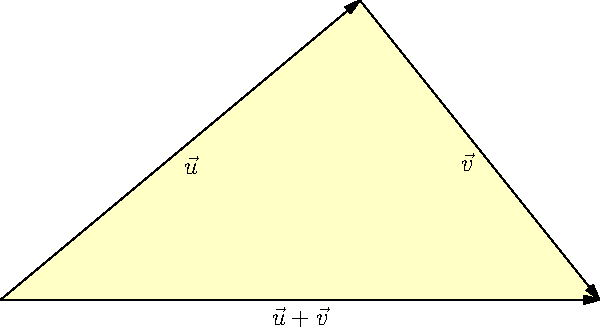
\includegraphics{./cap_algvet/pics/desigualdade_triangulo}
      \caption{Representação gráfica da desigualdade triangular: $\|\vec{u}+\vec{v}\|\leq \|\vct{u}\|+\|\vct{v}\|$}
      \label{fig:des_triang}
      %\setfloatalignment{b}% forces caption to be bottom-aligned
      \end{center}
   \end{figure}

Dica: Para mostrar a desigualdade triangular\index{desigualdade triangular}, entenda seu significado geométrico. Uma demonstração puramente algébrica pode ser feita, embora seja mais laboriosa. Veremos mais adiante que o conceito de produto escalar\index{produto escalar} permite simplificar os cálculos. 

A fim de simplificar a notação, a norma de um vetor $\vct{v}$ pode ser escrita simplesmente como $v$, ou seja
$$v=\|\vct{v}\|$$ 

Um vetor de norma 1 é chamado de vetor unitário\index{vetor unitário}. Todo vetor não nulo pode ser escrito na forma
\begin{equation}\label{decompversor}\vct{v}=v \hat{v}\end{equation}
onde $v$ é a norma de $\vct{v}$ e $\hat{v}$ é um vetor unitário dado por
\begin{equation}\label{defversor}\hat{v}=\frac{\vct{v}}{v}.\end{equation}
O vetor $\hat{v}$ é chamado de versor\index{versor} de $\vct{v}$. $\hat{v}$ é um vetor unitário que tem mesmo sentido e direção de $\vct{v}$.

A identidade (\ref{decompversor}) tem uma importante interpretação geométrica: todo vetor não nulo pode ser representado pelo seu módulo e por seu versor, que traz a informação de direção e sentido.  Os vetores $\vct{i}$, $\vct{j}$ e $\vct{k}$ são exemplos de versores. O vetor nulo é o único vetor ao qual não se pode associar direção e sentido únicos.


\begin{exer}Mostre que a norma de um versor conforme definido em (\ref{defversor}) é sempre unitária. 
\end{exer}

\begin{exer}\label{ex1uvw} Considere os vetores dados por $\vct{u}=\vct{i}+\vct{j}$, $\vct{v}=\vct{i}+2\vct{j}$ e $\vct{w}=\frac{1}{3}\vct{i}+\frac{1}{2}\vct{j}$. Represente estes vetores em um referencial euclidiano, calcule suas normas, calcule os versores associados $\hat{u}$, $\hat{v}$ e $\hat{w}$ e represente-os no mesmo gráfico.  
\end{exer}
Resp: $u=\sqrt{2}$, ~~ $v=\sqrt{5}$ ~e~ $w=\frac{\sqrt{13}}{{6}}$.~ $\hat{u}=\frac{\sqrt{2}}{2}\vct{i}+\frac{\sqrt{2}}{2}\vct{j}$,~~  $\hat{v}=\frac{\sqrt{5}}{5}\vct{i}+\frac{2\sqrt{5}}{5}\vct{j}$,~~ $\hat{w}=\frac{2\sqrt{13}}{13}\vct{i}+\frac{3\sqrt{13}}{13}\vct{j}$

\begin{exer} Considere o vetor $\vct{u}=\cos\theta \vct{i}+ \sin\varphi \vct{j}$. Mostre que este vetor é unitário e represente-o graficamente quando $\varphi=0$, $\varphi=\frac{\pi}{6}$, $\varphi=\frac{\pi}{2}$ e $\varphi={\pi}$ 
\end{exer}

\begin{exer} Considere o vetor $\vct{u}=\sin\theta \cos\varphi \vct{i}+ \sin\theta \sin\varphi \vct{j} + \cos\theta \vct{k}$. Verifique que este vetor é unitário e represente-o graficamente quando
\begin{itemize}
\item[a)] $\theta=0$
\item[b)] $\theta=\frac{\pi}{4}$ e $\varphi=\frac{\pi}{4}$
\item[c)] $\theta=\frac{\pi}{2}$ e $\varphi=\frac{\pi}{4}$
\item[d)] $\theta=\pi$

\end{itemize}
\end{exer}

\begin{exer}\label{probmaxmin} Seja $\vct{u}=u_1\vct{i} + u_2\vct{j}$ um vetor não nulo fixo no plano $xy$ e $\vct{v}=v\left(\cos\varphi \vct{i}+\sin\varphi \vct{j}\right)$ um vetor de norma fixa no plano $xy$. Considere a função $m(\varphi)=\|\vct{u}+\vct{v}\|$ e encontre o valor máximo e mínimo de $m(\varphi)$. Interprete o resultado.
\end{exer}

\begin{exer}\label{probdextro} Conforme observado no texto, um trio de vetores $\vct{u}$, $\vct{v}$ e $\vct{w}$ é dextrogiro se
\begin{equation*}
\det\left(\vct{u};\vct{v};\vct{w}\right)= \left|\begin{array}{ccc}
u_1&v_1&w_1\\
u_2&v_2&w_2\\
u_3&v_3&w_3
\end{array}
\right|>0.
\end{equation*}   
onde $\vct{u}=u_1\vct{i}+u_2\vct{j}+u_3\vct{k}$, $\vct{v}=v_1\vct{i}+v_2\vct{j}+v_3\vct{k}$ e $\vct{w}=w_1\vct{i}+w_2\vct{j}+w_3\vct{k}$. Faça o que se pede:
\begin{itemize}
\item [a)]Verifique que se $\vct{u}$, $\vct{v}$ e $\vct{w}$ forma um sistema dextrogiro então $\vct{v}$, $\vct{u}$ e $\vct{w}$ é levogiro.
\item [b)]Verifique que se $\vct{u}$, $\vct{v}$ e $\vct{w}$ forma um sistema dextrogiro então $\vct{v}$, $\vct{w}$ e $\vct{u}$ e $\vct{w}$, $\vct{u}$ e $\vct{v}$ são dextrogiros. 
\item [c)]Verifique que o trio $\vct{u}$, $\vct{v}$ e $\vct{w}$ é dextrogiro quando $\vct{u}=\vct{i}+\vct{j}$, $\vct{v}=-2\vct{i}+\vct{j}$ e $\vct{w}=\vct{i}+\vct{j}+\vct{k}$. 
\item [d)]Verifique que o trio $\vct{u}$, $\vct{v}$ e $\vct{w}$ é dextrogiro quando $\vct{u}=\vct{i}+\vct{j}$, $\vct{v}=-2\vct{i}+\vct{j}$ e $\vct{w}=\vct{i}$. Interprete graficamente.
\end{itemize}
\end{exer}

%\begin{exer} Seja $\vct{u}=u_1\vct{i} + u_2\vct{j} + u_3\vct{k}$ um vetor não nulo fixo e $\vct{v}=v\left(\sin\theta \cos\varphi \vct{i}+ \sin\theta \sin\varphi \vct{j} + \cos\theta \vct{k}\right)$ um vetor de norma fixa. Considere a função $m(\varphi,\theta)=\|\vct{u}+\vct{v}\|$ e encontre o valor máximo e mínimo de $m(\varphi,\theta)$. Interprete o resultado.
%\end{exer}



\begin{figure}%[20\baselineskip]
\begin{center}
\includegraphics{./cap_algvet/pics/latitude_longitude2}
      \caption{Representação gráfica do sistema de coordenadas geográficas.}
      \label{fig:latlong}
      \end{center}
  \end{figure}

\begin{exer} 
Considere um sistema de coordenadas cartesianas dextrogiro construído da seguinte forma:

\begin{itemize}
\item O centro da Terra coincide com a origem do sistema.
\item O extremo norte da Terra intercepta o eixo $z$ em valores positivos.
\item O observatório de Greenwich está sob plano $xz$ com $x>0$.
\end{itemize}
Considere a superfície terrestre com uma esfera de raio $R_{\oplus}$. Denote a longitude\index{longitude} por $\lambda$ e a latitude\index{latitude} por $\phi$. Convecione como positivas a longitude leste  e a latitude norte. Veja figura \ref{fig:latlong}. Seja $\vct{r}=x\vct{i}+y\vct{j}+z\vct{k}$ o vetor que representa um ponto sobre a superfície da Terra. Responda:
\begin{itemize}
\item[a)] Qual a norma do vetor $\vct{r}$?
\item[b)] Qual é o valor da componentes $x$, $y$ e $z$ de $\vct{r}$ em termos de $\lambda$ e $\phi$? 
\item[c)] Seja $d$ a distância entre dois pontos sobre a superfície terrestre. Use a lei dos cossenos\footnote{Seja um triângulo de lados $a$, $b$ e $c$ e seja $\theta$ o ângulo entre os lados de comprimento $a$ e $b$, então $c^2=a^2+b^2-2ab\cos\theta.$ Ver também figura \ref{leicossenos} na página \pageref{leicossenos}.} para mostrar que distância $\delta$ sobre a superfície esférica entre esses mesmos dois pontos é dada por
$$\delta=R_\oplus \cos^{-1}\left(1-\frac{d^2}{2R_\oplus^2}\right)$$
Interprete os casos particulares $d=0$ e $d=2R_\oplus$. 
\item[d)] Considerando $R_\oplus=6378Km$ e os seguintes valores para as coordenadas geográficas de Porto Alegre, Londres e Tóquio, construa uma tabela com os valores de $\lambda$ e $\phi$ e as coordenadas $xyz$ em quilômetros de cada uma dessas cidades.
\begin{table}[h]
	\centering
		\begin{tabular}{|l|l|l|}
		\hline
	  Localidade & Latitude & Longitude\\ 
		\hline
		Porto Alegre & $30^\circ~ 01{'}~58{''}$S & $51^\circ  13{'}~48{''}$O\\ 		
  	\hline
		Londres & $51^\circ~ 30{'}~28{''}$N & $0^\circ~ 7{'}~41{''}$O\\ 		
  	\hline
  	Tóquio & $35^\circ~ 41{'}~22{''}$N & $139^\circ ~41{'}~30{''}$L\\ 		
  	\hline	
		\end{tabular}
	\caption{Coordenadas geográficas de algumas cidades.}
	\label{tabcidades}
\end{table}
\item[e)] Contrua uma tabela com as distâncias em linha reta e sobre a superfície da Terra entre cada uma dessas cidades.
\item[f)] As seguintes coordenadas indicam locais de grande importância cultural ou turística, identifique-os:
\begin{table}[htp]
	\centering
		\begin{tabular}{|l|l|l|l|}
		\hline
Localidade &	  x & y & z\\ 
		\hline
1&		4192,872Km & 168Km & 4803,175Km\\
		\hline
2&		1175,603Km&	5550,889Km&	2912,813Km\\
		\hline
3&   3996,282Km&	-127,418Km&	4969,143Km\\
  	\hline	
		\end{tabular}
	\caption{Coordenadas geográficas de três localidades incógnitas.}
	\label{tabmonumentos}
\end{table}
\end{itemize}   
\end{exer}


% 
% \begin{figure}[h]
% \begin{center}
% \includegraphics[width=.6\linewidth]{./cap_algvet/pics/latitude_longitude2}
%       \caption{Representação gráfica do sistema de coordenadas geográficas.}
%       \label{fig:latlong}
%       \end{center}
%   \end{figure}



     

\begin{table}[h]
Resp: a) $r=R_\oplus$ b)
 $x=R_\oplus \cos\phi \cos\lambda$, $y=R_\oplus \cos\phi\sin\lambda$ e $z=R_\oplus \sin\phi$
	\centering
		\begin{tabular}{|l|l|l|l|l|l|}
		\hline
	  Localidade & $\phi$ & $\lambda$ & $x$ & $y$ & $z$\\ 
		\hline
		Porto Alegre & $-30,0328^\circ$ & $-51,23^\circ$& $3457,65$&$-4305,07$& $-3192,16$\\ 		
  	\hline
		Londres & $51,5078^\circ$ & $-0,0781^\circ$&3969,71&-5,41&4992,02\\ 		
  	\hline
  	Tóquio & $35,6894^\circ$ & $139,6917^\circ$&3950,26&3351,05&3720,87\\ 		
  	\hline	
		\end{tabular}
	\caption{Coordenadas geográficas  e cartesianas de algumas cidades - solução do item d.}
\vspace{10pt}
		\begin{tabular}{|l|l|l|}
		\hline
	  Localidades & Distância em linha reta & Distância sobre a superfície esférica \\ 
		\hline
		Porto Alegre-Londres & 9260Km & 10360Km\\ 		
  	\hline
  	Porto Alegre-Tóquio & 12700Km&18840Km\\ 		
  	\hline
		Tóquio-Londres &8695Km &9570Km\\ 		
  	\hline		
		\end{tabular}
	\caption{Distância entre as cidades - solução do item e.}

\vspace{10pt}	
		\begin{tabular}{|l|l|l|l|}
		\hline
Localidade &	  $\lambda$ & $\phi$& Identificação\\ 
		\hline
1&		$48^\circ 51{'}30{''}$N &	$0^\circ 02{'}24{''}$L & \\
	\hline
2&	  $27^\circ 10{'}27{''}$N & 	$0^\circ 58{'}42{''}$L & \\
	\hline
3&	  $51^\circ 10{'}44{''}$N & $0^\circ 01{'}55{''}$W&  \\
		\hline		
		\end{tabular}
	\caption{Solução do item f}
\end{table}



\section{Ângulo entre vetores e o produto escalar}
Na seção anterior, começamos a trabalhar com vetores no espaço euclidiano. No entanto, até o momento não lidamos explicitamente com ângulos entre vetores. Introduziremos primeiramente o conceito de produto escalar ou produto interno entre vetores. O produto escalar\index{produto escalar} é uma operação que liga um par de vetores a um escalar. O produto escalar entre os vetores $\vct{u}$ e $\vct{v}$  é denotado por $\vct{u}\cdot \vct{v}$ e é definida no espaço euclidiano tridimensional como:
\begin{equation}\label{defprodesc}\vct{u}\cdot\vct{v}=u_1v_1+u_2v_2+u_3v_3\end{equation}




Considere os vetores $\vct{u}$, $\vct{v}$ e $\vct{w}$ relacionados por $$\vct{w}=\vct{u}-\vct{v}.$$
\begin{figure}\begin{center}
        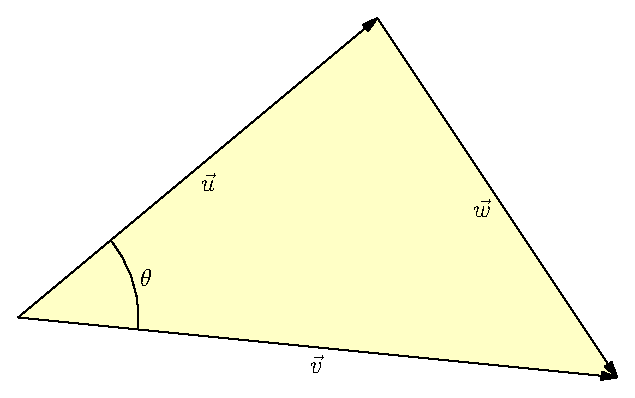
\includegraphics[width=\textwidth]{./cap_algvet/pics/cossenos} %
    \caption{Lei dos cossenos: $\|\vct{w}\|^2=\|\vct{u}\|^2+\|\vec{v}\|^2-2~\!\|\vec{u}\|~\!\|\vec{v}\|\cos\theta$}\label{leicossenos}
    \end{center}
\end{figure}
Este trio de vetores pode ser intepretado como os três lados de um triângulo como na figura \ref{leicossenos}. Da lei dos cossenos, sabemos que a seguinte relação é satisfeita:
 $$w^2=u^2+v^2-2uv\cos\theta$$
supondo $u\neq 0$ e $v\neq 0$, temos
$$\cos\theta = \frac{w^2-u^2-v^2}{2uv}.$$
Usamos agora a definição de norma de um vetor dada em (\ref{defnorma}):
\begin{eqnarray*}
u^2&=&u_1^2+u_2^2+u_3^2\\
v^2&=&v_1^2+v_2^2+v_3^2\\
w^2&=&w_1^2+w_2^2+w_3^2=\left(u_1-v_1\right)^2+\left(u_2-v_2\right)^2+\left(u_3-v_3\right)^2\\
\end{eqnarray*}
Simplificando, temos:
$$\cos\theta = \frac{w^2-u^2-v^2}{2uv}=\frac{u_1v_1+u_2v_2+u_3v_3}{uv}=\frac{\vct{u}\cdot\vct{v}}{uv}$$
Esta última expressão nos permite escrever
\begin{equation}\label{defintriprodesc}
\vct{u}\cdot\vct{v}=uv\cos\left(\vct{u},\vct{v}\right)=uv\cos\theta
\end{equation}
onde $\cos\left(\vct{u},\vct{v}\right)$ indica o cosseno do ângulo entre os vetores $\vct{u}$ e $\vct{v}$.
\begin{obs}Neste momento, o leitor deve observar que a definição que demos originalmente para o produto escalar em (\ref{defprodesc}) dependia fortemente do sistema de coordenadas escolhido. No entanto, a identidade (\ref{defintriprodesc}) mostra que o valor do produto escalar depende apenas da norma dos vetores envolvidos e do ângulo entre esses vetores, ou seja,  (\ref{defintriprodesc}) pode ser usado como uma definição intrínseca (que não depende da escolha do sistema de coordenadas) de produto escalar. \end{obs}
\begin{obs}O produto escalar do vetor nulo $\vct{0}$ por qualquer vetor é zero.\end{obs}


O produto escalar satisfaz as seguintes propriedades:
%\begin{formulario}
\begin{subequations}\label{proprodesc}
\begin{align}
\vct{u}\cdot\vct{v}&=\vct{v}\cdot\vct{u},&\mytext{(Comutatividade)}\label{propprodesccom}\\
\vct{u}\cdot\left(\alpha\vct{v}+\beta \vct{w}\right)&=\alpha(\vct{u}\cdot\vct{v})+\beta(\vct{u}\cdot\vct{w}),\hspace{-5cm}&\mytext{(Linearidade)}\label{propprodesclin}\\
\vct{u}\cdot\vct{u}&=u^2,&\mytext{(Respeito à norma)}\label{propprodescnorma}\\
\left|\vct{u}\cdot\vct{v}\right|&\leq uv,&\mytext{(Desigualdade de Cauchy-Schwarz)}\label{propprodesccauchy}
\end{align}
\end{subequations}
%\end{formulario}
As propriedades (\ref{propprodesccom}), (\ref{propprodesclin}) e (\ref{propprodescnorma}) podem ser trivialmente demonstradas diretamente a partir da definição de produto escalar dada em (\ref{defprodesc}).
\begin{exer} Demonstre essas três propriedades.
\end{exer}
Observe que $\alpha(\vct{u}\cdot\vct{v})=(\alpha~\!\vct{u})\cdot\vct{v}$ pelo que podemos escrever $\alpha~\!\vct{u}\cdot\vct{v}$ sem risco de ambiguidade.  
\begin{exer} Use (\ref{propprodesccom}) e  (\ref{propprodesclin}) para mostrar a seguinte propriedade:
$$
\left(\alpha\vct{u}+\beta \vct{v}\right)\cdot \vct{w}=\alpha (\vct{u}\cdot\vct{w})+ \beta (\vct{v}\cdot\vct{w})
$$

\end{exer}
~~ \\

A \underline{desigualdade de Cauchy-Schwarz}\index{desigualdade de Cauchy-Schwarz} (\ref{propprodesccauchy}) pode ser demonstrada a partir de (\ref{defintriprodesc}) uma vez que $$-1\leq \cos\theta \leq 1.$$
No entanto, uma demonstração puramente algébrica pode ser dada a partir das propriedades (\ref{propprodesccom}), (\ref{propprodesclin}) e (\ref{propprodescnorma}). Dada a beleza desta demonstração e da possibilidade de generalização, apresentamo-na a seguir:

Consideramos primeiramente os versores $\hat{u}$ e $\hat{v}$ definidos em (\ref{defversor}) e calculamos
\begin{eqnarray*}
\|\hat{u}+\hat{v}\|^2 &=& \left(\hat{u}+\hat{v}\right)\cdot \left(\hat{u}+\hat{v}\right) = 2+2\hat{u}\cdot\hat{v} \\
\|\hat{u}-\hat{v}\|^2 &=& \left(\hat{u}-\hat{v}\right)\cdot \left(\hat{u}-\hat{v}\right) = 2-2\hat{u}\cdot\hat{v} 
\end{eqnarray*}
onde usamos que $\hat{u}\cdot\hat{u}=\hat{v}\cdot\hat{v}=1$ posto que a norma de um versor é sempre 1. Agora observamos que $\|\hat{u}+\hat{v}\|^2\geq 0 $ e $\|\hat{u}-\hat{v}\|^2\geq 0 $, pelo que temos:
$$-1\leq \hat{u}\cdot\hat{v} \leq 1$$
O que implica $|\hat{u}\cdot\hat{v}|\leq 1$. Como $\vct{u}=u\hat{u} $ e $\vct{v}=v\hat{v}$, temos
$$|\vct{u}\cdot\vct{v}|\leq uv$$ 

Observamos que com uma demontração puramente algébrica para a desigualdade de Cauchy-Schwarz, podemos derivar uma demonstração puramente algébrica da \underline{desigualdade triangular} (\ref{propnormatri}). Ver também a discussão do excício \ref{exnorma}. Para tal considere a seguinte identidade:
$$\|\vct{u}+\vct{v}\|^2=\left(\vct{u}+\vct{v}\right)\cdot \left(\vct{u}+\vct{v}\right) = u^2+2\vct{u}\cdot\vct{v}+v^2$$
Como $\vct{u}\cdot\vct{v}\leq |\vct{u}\cdot\vct{v}|\leq uv$, temos:
$$\|\vct{u}+\vct{v}\|^2\leq u^2+2uv+v^2=(u+v)^2$$
Extraindo a raiz quadrada de ambos os lados, temos:
$$\|\vct{u}+\vct{v}\|\leq (u+v)=\|\vct{u}\|+\|\vct{v}\|$$
\\~\\
Dois vetores não nulos $\vct{u}$ e $\vct{v}$ são dito ortogonais\index{vetores ortogonais} se o ângulo entre eles é $90^\circ$, ou seja, se $\cos\left(\vct{u},\vct{v}\right)=0$. De (\ref{defintriprodesc}), isto acontece quando $\vct{u}\cdot\vct{v}=0$. Usamos o símbolo $\bot$ para denotar a ortogonalidade:
\begin{eqnarray}\vct{u}\bot \vct{v}\Longleftrightarrow \vct{u}\cdot\vct{v}=0\label{deforto}
\end{eqnarray}

Em especial os vetores unitários $\vct{i}$, $\vct{j}$ e $\vct{k}$ são ortogonais, ou seja: $$\vct{i}\cdot \vct{j}=\vct{i}\cdot \vct{k}=\vct{j}\cdot \vct{k}=0.$$

\begin{exer} Considere os vetores dados por $\vct{u}=\vct{i}+\vct{j}$, $\vct{v}=\vct{i}+2\vct{j}$ e $\vct{w}=\frac{1}{3}\vct{i}+\frac{1}{2}\vct{j}$ conforme exercício \ref{ex1uvw}. Calcule o ângulo entre esses vetores.  
\end{exer}
Resp: $18,43^\circ$, $11,3^\circ$ e  $7,13^\circ$
\begin{exer} Mostre que se $\alpha$ e $\beta$ são escalares diferentes de zero e $\vct{u}$ e $\vct{v}$ são vetores não nulos, então $$\cos\left(\alpha\vct{u},\beta\vct{v}\right)=\cos\left(\vct{u},\vct{v}\right).$$
Interprete geometricamente esta identidade.
\end{exer}


\begin{exer}Mostre que se $\vct{u}=u_1\vct{i}+u_2\vct{j}+u_3\vct{k}$ então $u_1=\vct{u}\cdot\vct{i}$, $u_2=\vct{u}\cdot\vct{j}$ e $u_3=\vct{u}\cdot\vct{k}$. Conclua que
$$\vct{u}=\left(\vct{u}\cdot\vct{i}\right) \vct{i}+\left(\vct{u}\cdot\vct{j}\right) \vct{j}+\left(\vct{u}\cdot\vct{k}\right) \vct{k}.$$

\end{exer}

\begin{exer}\label{exort1}Sejam $\vct{u}=\frac{\sqrt{2}}{2}\left(\vct{i}+\vct{j}\right)$ e $\vct{v}=\frac{\sqrt{2}}{2}\left(\vct{i}-\vct{j}\right)$. Mostre que estes vetores são unitários e ortogonais entre si. Encontre dois vetores unitários distintos ortogonais tanto a $\vct{u}$ quanto a $\vct{v}$.
\end{exer}
Resp: $-\vct{k}$ e $\vct{k}$.

\begin{exer}\label{exort2} Sejam $\vct{u}=2\vct{i}+\vct{j}+\vct{k}$ e $\vct{v}=2\vct{i}-\vct{j}-\vct{k}$. Mostre que estes vetores são ortogonais entre si. Encontre dois vetores unitários distintos ortogonais tanto a  $\vct{u}$ como a $\vct{v}$.
\end{exer}
Resp: $\frac{\sqrt{2}}{2}\left(\vct{j}-\vct{k}\right)$ e $\frac{\sqrt{2}}{2}\left(-\vct{j}+\vct{k}\right)$.

\begin{exer} Encontre três vetores $\vct{u}$, $\vct{v}$ e $\vct{w}$ tais que:
\begin{itemize}
\item [a)] $\left(\vct{u}\cdot\vct{v}\right)\vct{w}=\vct{0}$ mas $\vct{u}\left(\vct{v}\cdot\vct{w}\right)\neq \vct{0}$ 
\item [b)] $\left(\vct{u}\cdot\vct{v}\right)\vct{w}\neq \vct{u}\left(\vct{v}\cdot\vct{w}\right)$ e ambos não nulos. 
\end{itemize}
\end{exer}

Exemplos de respostas: a) $\vct{u}=\vct{i}$, $\vct{v}=\vct{j}$ e $\vct{w}=\vct{j}$. b) $\vct{u}=\vct{i}$, $\vct{v}=\vct{i}+\vct{j}$ e $\vct{w}=\vct{j}$.

\begin{exer} Sejam os vetores $\vct{u}=\cos(\theta_1)\vct{i}+\sin(\theta_1)\vct{j}$ e $\vct{v}=\cos(\theta_2)\vct{i}+\sin(\theta_2)\vct{j}$ então
$$\cos\left(\vct{u},\vct{v}\right)=\cos(\theta_1-\theta_2).$$
Conclua que o ângulo $\theta$ entre $\vct{u}$ e $\vct{v}$ é dado por
$$\theta=\left\{
\begin{array}{ll}
|\theta_1-\theta_2|,& |\theta_1-\theta_2|\leq 180^\circ\\
360^\circ-|\theta_1-\theta_2|,& |\theta_1-\theta_2|> 180^\circ\\
\end{array}
\right.$$ 
contanto que $\theta_1$ e $\theta_2$ estejam entre $0$ e $360^\circ$.
Interprete geometricamente este resultado.
\end{exer}

\begin{exer}Seja $\vct{u}$ um vetor não nulo fixo e $\vct{v}$ um vetor de norma não nula fixa. Mostre que $\|\vct{u}+\vct{v}\|$ tem um ponto de máximo quando $\hat{u}=\hat{v}$ e um ponto de mínimo quando $\hat{u}=-\hat{v}$. Interprete o resultado geometricamente e compare com o problema (\ref{probmaxmin}). 
\end{exer}
 Dica: $\|\vct{u}+\vct{v}\|^2=u^2+v^2+2\vct{u}\cdot\vct{v}$ e (\ref{defintriprodesc}).

\section{O produto vetorial}
Além do produto escalar entre vetores, definimos também o produto vetorial\index{produto vetorial}. Enquanto o produto escalar de dois vetores é um escalar, o produto vetorial é um terceiro vetor. O produto vetorial entre $\vct{u}=u_1\vct{i}+u_2\vct{j}+u_3\vct{k}$ e $\vct{v}=v_1\vct{i}+v_2\vct{j}+v_3\vct{k}$ é denotado $\vct{u}\times\vct{v}$ e é definido em coordenadas cartesianas como:
\begin{equation}\label{defprodvec} \vct{u}\times\vct{v}=\left(u_2v_3-u_3v_2\right)\vct{i}+\left(u_3v_1-u_1v_3\right)\vct{j}+\left(u_1v_2-u_2v_1\right)\vct{k}
\end{equation}
A definição de produto vetorial pode parecer à primeira vista arbitrária e fortemente dependente do sistema de coordenadas escolhido. No entanto, mostraremos que  o produto vetorial admite uma formulação intrínseca, ou seja, que não depende do sistema de coordenadas escolhido. Ademais, veremos que tanto o produto escalar como o produto vetorial surgem naturalmente no estudo da física clássica.

O produto vetorial possui as seguintes propriedades:
\begin{subequations}\label{propprodvec}
\begin{align}
\vct{u}\times\vct{v}&=-\vct{v}\times\vct{u},&\mytext{(Anticomutatividade)}\label{propprodvecanticom}\\
\left(\alpha \vct{u}+ \beta\vct{v}\right)\times\vct{w}&=\alpha\left(\vct{u}\times\vct{w}\right)+\beta\left(\vct{v}\times\vct{w}\right),&\mytext{(Linearidade à esquerda)}\label{propprodveclin1}\\
\vct{u}\times\left(\alpha \vct{v}+ \beta\vct{w}\right)&=\alpha\left(\vct{u}\times\vct{v}\right)+\beta\left(\vct{u}\times\vct{w}\right),&\mytext{(Linearidade à direita)}\label{propprodveclin2}\\
\left(\vct{u}\times \vct{v}\right)\cdot \vct{u}&=\left(\vct{u}\times \vct{v}\right)\cdot \vct{v}=0,&\mytext{(Ortogonalidade)}\label{propprodvecorto}\\
\left\|\vct{u}\times \vct{v}\right\|&=uv\sin(\vct{u},\vct{v})
.&\mytext{(Norma)}\label{propprodvecnorma}\\
\det\left(\vct{u}; \vct{v};\vct{u}\times \vct{v}\right)&=u^2v^2\sin^2(\vct{u},\vct{v})>0
.&\mytext{(Orientação dextrogira)}\label{propprodvecorient}
\end{align}
\end{subequations}
Nas duas últimas propriedades, $\sin(\vct{u},\vct{v})$ denota o seno do ângulo entre os vetores $\vct{u}$ e $\vct{v}$. Observa-se que quando $\vct{u}$ ou $\vct{v}$ é nulo, este ângulo não está bem definido, estas identidades devem ser então interpretadas como $\left\|\vct{u}\times \vct{v}\right\|=0$ e $\det\left(\vct{u}; \vct{v};\vct{u}\times \vct{v}\right)=0$.

A última propriedade significa que o trio $\vct{u}$, $\vct{v}$ e $\vct{u}\times\vct{v}$ forma um sistema dextrogiro.

\begin{exer} Mostre as propriedades (\ref{propprodvecanticom}), (\ref{propprodveclin1}) e (\ref{propprodveclin2}).  
\end{exer}
A propriedade da ortogonalidade pode ser demonstrada diretamente da definição de produto vetorial e produto escalar:
\begin{eqnarray*}\left(\vct{u}\times \vct{v}\right)\cdot \vct{u}&=&\left[\left(u_2v_3-u_3v_2\right)\vct{i}+\left(u_3v_1-u_1v_3\right)\vct{j}+\left(u_1v_2-u_2v_1\right)\vct{k}\right]\left(u_1\vct{i}+u_2\vct{j}+u_3\vct{k}\right)\\
&=&\left(u_2v_3-u_3v_2\right)u_1+\left(u_3v_1-u_1v_3\right)u_2+\left(u_1v_2-u_2v_1\right)u_3=0
\end{eqnarray*}
igualmente temos:
\begin{eqnarray*}\left(\vct{u}\times \vct{v}\right)\cdot \vct{v}&=&\left[\left(u_2v_3-u_3v_2\right)\vct{i}+\left(u_3v_1-u_1v_3\right)\vct{j}+\left(u_1v_2-u_2v_1\right)\vct{k}\right]\left(v_1\vct{i}+v_2\vct{j}+v_3\vct{k}\right)\\
&=&\left(u_2v_3-u_3v_2\right)v_1+\left(u_3v_1-u_1v_3\right)v_2+\left(u_1v_2-u_2v_1\right)v_3=0
\end{eqnarray*}
Para provar a propriedade (\ref{propprodvecnorma}), mostraremos primeiramente a seguinte (interessante) identidade:
\begin{equation}\label{identnorma}\left\|\vct{u}\times \vct{v}\right\|^2+\left|\vct{u}\cdot \vct{v}\right|^2=u^2v^2
\end{equation}
Da definição de norma e de produto vetorial temos:
\begin{eqnarray}\label{calcnormaprodvec}
\left\|\vct{u}\times \vct{v}\right\|^2&=&\left\|\left(u_2v_3-u_3v_2\right)\vct{i}+\left(u_3v_1-u_1v_3\right)\vct{j}+\left(u_1v_2-u_2v_1\right)\vct{k}\right\|^2\nonumber\\
&=&\left(u_2v_3-u_3v_2\right)^2+\left(u_3v_1-u_1v_3\right)^2+\left(u_1v_2-u_2v_1\right)^2\nonumber\\
&=&\left(u_2^2v_3^2-2u_2u_3v_2v_3+u_3^2v_2^2\right)+\left(u_3^2v_1^2-2u_1u_3v_1v_3+u_1^2v_3^2\right) \nonumber\\
&+&\left(u_1^2v_2^2-2u_1u_2v_1v_2+u_2^2v_1^2\right).
\end{eqnarray}
Da definição de norma e de produto escalar temos:
\begin{eqnarray*}
\left|\vct{u}\cdot \vct{v}\right|^2&=&\left(u_1v_1+u_2v_2+u_3v_3\right)^2=u_1^2v_1^2+u_2^2v_2^2+u_3^2v_3^2+2u_1u_2v_1v_2+2u_1u_3v_1v_3+2u_2u_3v_2v_3.
\end{eqnarray*}
Somando estas últimas duas expressões, simplificando e reagrupando termos, chegamos ao resultado desejado:
\begin{eqnarray*}
\left\|\vct{u}\times \vct{v}\right\|^2+\left|\vct{u}\cdot \vct{v}\right|^2&=&\left(u_1v_1+u_2v_2+u_3v_3\right)^2\\
&=&u_1^2v_1^2+u_1^2v_2^2+u_1^2v_3^2+u_2^2v_1^2+u_2^2v_2^2+u_2^2v_3^2+u_3^2v_1^2+u_3^2v_2^2+u_3^2v_3^2\\
&=&\left(u_1^2+u_2^2+u_3^2\right)\left(v_1^2+v_2^2+v_3^2\right)=u^2v^2.
\end{eqnarray*}
Agora que dispomos da identidade (\ref{identnorma}), usamos (\ref{defintriprodesc}) para escrever 
\begin{equation*}\left\|\vct{u}\times \vct{v}\right\|^2=u^2v^2-\left|\vct{u}\cdot \vct{v}\right|^2=u^2v^2-\left[uv\cos\left(\vct{u},\vct{v}\right)\right]^2=u^2v^2\left[1-\cos^2\left(\vct{u},\vct{v}\right)\right]=u^2v^2\sin^2\left(\vct{u},\vct{v}\right)
\end{equation*}
Extraímos a raiz quadrada, observando que $\sin\left(\vct{u},\vct{v}\right)\geq 0$ e obtemos o resultado desejado (\ref{propprodvecnorma}).
Um caso particular importante é quando os vetores $\vct{u}$ e $\vct{v}$ estão na mesma direção. Como $\sin 0= \sin 180^\circ=0$, o produto vetorial de dois vetores paralelos é $\vct{0}$.  
Para demonstrar a propriedade (\ref{propprodvecorient}), calculamos o determinante envolvido
\begin{eqnarray*}
\det\left(\vct{u};\vct{v};\vct{u}\times\vct{v}\right)&=&\left|
\begin{array}{ccc}
u_1 & v_1 & \left(u_2v_3-u_3v_2\right)\\  
u_2 & v_2 & \left(u_3v_1-u_1v_3\right)\\ 
u_3 & v_3 &  \left(u_1v_2-u_2v_1\right)
\end{array}
\right|\\
&=&\left(u_1^2v_2^2-u_1u_2v_1v_2\right)+\left(u_3^2v_1^2-u_1u_3v_1v_3\right)+\left(u_2^2v_3^2-u_2u_3v_2v_3\right)\\
&-&\left(u_1u_2v_1v_2-u_2^2v_1^2\right)-\left(u_1u_3v_1v_3-u_1^2v_3^2\right)-\left(u_2u_3v_2v_3-u_3^2v_2^2\right)
\end{eqnarray*}
\begin{figure}%[-30\baselineskip]
     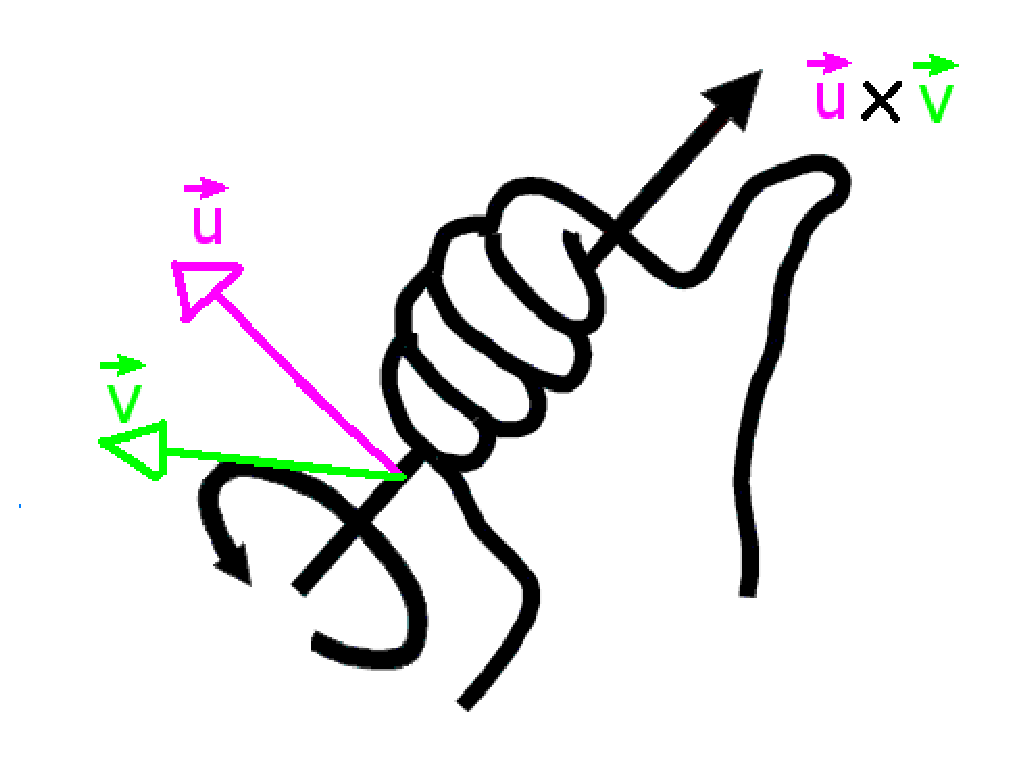
\includegraphics[width=\textwidth]{./cap_algvet/pics/R_mao_dir.eps}
      \caption{Regra da mão direita. }
      %\label{fig:marginfig}
      %\setfloatalignment{b}% forces caption to be bottom-aligned
  \end{figure}


Agora basta observar que esta expressão é idêntica a (\ref{calcnormaprodvec}), ou seja, $\|\vct{u}\times\vct{v}\|^2$ e portanto o determinante $\det\left(\vct{u};\vct{v};\vct{u}\times\vct{v}\right)$ é positivo. 

A importância desta propriedade está no fato que se $\vct{w}=\vct{u}\times \vct{v}$ então o trio de vetores $\vct{u}$, $\vct{v}$ e $\vct{w}$ forma um sistema dextrogiro. Além disso, por causa da propriedade (\ref{propprodvecorto}), $\vct{w}$ deve ser ortogonal tanto aos vetores $\vct{u}$, $\vct{v}$. Finalmente, observando a propriedade da norma (\ref{propprodvecnorma}), podemos estabelecer a seguinte identidade para o produto vetorial de dois vetores não colineares $\vct{u}$ e $\vct{v}$:
\begin{equation}
\vct{u}\times\vct{v}=uv\sin\left(\vct{u},\vct{v}\right)\hat{e}
\end{equation}
onde o versor $\hat{e}$ é ortogonal ao plano gerado por $\vct{u}$ e $\vct{v}$ e forma um sistema dextrogiro com eles.  

\begin{figure}%[10\baselineskip]
\begin{center}
     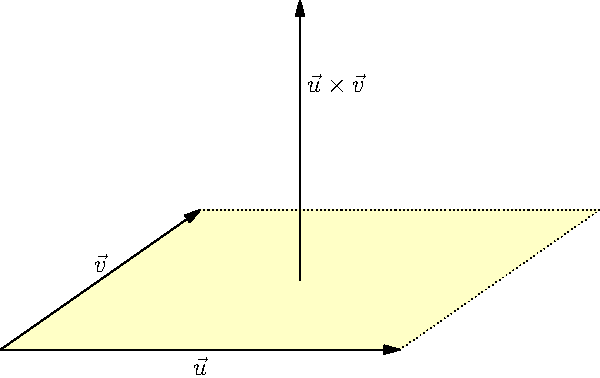
\includegraphics[width=\textwidth]{./cap_algvet/pics/prod_vec_paralelogramo}
      \caption{Interpretação geométrica do produto vetorial.}\label{fig:prod_paralelo}
      %\label{fig:marginfig}
      %\setfloatalignment{b}% forces caption to be bottom-aligned
      \end{center}
  \end{figure}

  A norma do produto vetorial entre os vetores $\vct{u}$ e $\vct{v}$ pode ser interpretada como a área do paralelogramo cujos lados são $\vct{u}$ e $\vct{v}$ (ver figura \ref{fig:prod_paralelo}. A direção do produto vetorial é então ortogonal ao plano gerado por  $\vct{u}$ e $\vct{v}$  e o sentido é dado pela regra da mão direita.


%\begin{figure}[h!]
%  \begin{center}
 % \vspace{-20pt}
    %\includegraphics[width=0.5\textwidth]{./cap_algvet/pics/prod_vec_mao_dir}
 % \end{center}
  %\vspace{-20pt}
  %\caption{Interpretação geométrica do produto vetorial.}\label{prod_paralelo}

%\end{figure}

A definição de produto vetorial dada em (\ref{defprodvec}) pode ser mais facilmente lembrada através do seguinte determinante formal:
\begin{equation}\label{detprodvec}
\vct{u}\times\vct{v}=\left|\begin{array}{ccc}
\vct{i}&\vct{j}&\vct{k}\\
u_1 & u_2 & u_3\\
v_1 & v_2 & v_3\\
\end{array}
\right|
\end{equation}
que pode ser calculado pela regra de Sarrus.

O produto vetorial entre os vetores unitários $\vct{i}$, $\vct{j}$ e $\vct{k}$ pode ser obtido da definição (\ref{defprodvec}) ou da caracterização geométrica do produto vetorial:

\begin{align}\label{prodvecunit}
\vct{i}\times \vct{i}&=\vct{0},\qquad & \vct{i}\times \vct{j}&=\vct{k},\qquad &\vct{i}\times \vct{k}&=-\vct{j}\nonumber\\
\vct{j}\times \vct{i}&=-\vct{k},\qquad & \vct{j}\times \vct{j}&=\vct{0},\qquad& \vct{j}\times \vct{k}&=\vct{i}\nonumber\\
\vct{k}\times \vct{i}&=\vct{j},\qquad &\vct{k}\times \vct{j}&=-\vct{i},\qquad &\vct{k}\times \vct{k}&=\vct{0}
\end{align}

\begin{exer} Seja $\vct{u}=\vct{i}+2\vct{j}$ e $\vct{v}=3\vct{i}-2\vct{j}$, calcule o vetor $\vct{w}=\vct{u}\times\vct{v}$.
\end{exer}
{\bf Solução 1} Calcularemos primeiramente usando o determinante (\ref{detprodvec}):
\begin{eqnarray*}\vct{w}&=&\left|\begin{array}{ccc}
\vct{i}&\vct{j}&\vct{k}\\
u_1 & u_2 & u_3\\
v_1 & v_2 & v_3\\
\end{array}
\right|=\left|\begin{array}{ccc}
\vct{i}&\vct{j}&\vct{k}\\
1 & 2 & 0\\
3 & -2& 0\\
\end{array} \right|\\
&=&\vct{i}(0-0)+\vct{j}(0-0)+\vct{k}(-2-6)\\
&=&-8\vct{k}
\end{eqnarray*}

{\bf Solução 2} Calcularemos usando as propriedades (\ref{propprodvec}) e as relações (\ref{prodvecunit}):
\begin{eqnarray*}\vct{w}&=&\vct{u}\times\vct{v}= \left(\vct{i}+2\vct{j}\right)\times\left(3\vct{i}-2\vct{j}\right)\\
&=&3(\vct{i}\times\vct{i})-2(\vct{i}\times\vct{j})+6(\vct{j}\times\vct{i})-4(\vct{j}\times\vct{j})\\
&=&3~\!\vct{0}-2~\!\vct{k}-6~\!\vct{k}-4~\!\vct{0}\\
&=&-8\vct{k}
\end{eqnarray*}


\begin{exer} Refaça os exercícios \ref{exort1} e \ref{exort2} usando o conceito de produto vetorial.
\end{exer}

\begin{exer}\label{prodvecnaoassoc} Encontre três vetores $\vct{u}$, $\vct{v}$ e $\vct{w}$ tais que $\vct{u}\times\left(\vct{v}\times\vct{w}\right)\neq \left(\vct{u}\times\vct{v}\right)\times \vct{w}$. 
\end{exer}
Exemplo de resposta: $\vct{u}=\vct{i}$, $\vct{v}=\vct{i}$ e $\vct{w}=\vct{k}$.

\begin{exer} Simplifique as seguintes expressões:
\begin{itemize}
\item[a)] $\vct{u}\times\vct{u}$
\item[b)] $\vct{u}\times\hat{u}$
\item[c)] $\vct{u}\cdot\vct{u}$
\item[d)] $\vct{u}\cdot\hat{u}$
\item[e)] $\left(\vct{u}+\vct{v}\right)\cdot\left(\vct{u}+\vct{v}\right)$
\item[f)] $\left(\vct{u}+\vct{v}\right)\times\left(\vct{u}+\vct{v}\right)$
\item[g)] $\left(\vct{u}-\vct{v}\right)\cdot\left(\vct{u}-\vct{v}\right)$
\item[h)] $\left(\vct{u}-\vct{v}\right)\times\left(\vct{u}-\vct{v}\right)$
\item[i)] $\left(\vct{u}+\vct{v}\right)\cdot\left(\vct{u}-\vct{v}\right)$
\item[j)] $\left(\vct{u}+\vct{v}\right)\times\left(\vct{u}-\vct{v}\right)$
\end{itemize}
\end{exer}
Resp: $\vct{0}$,$\vct{0}$,$u^2$,$u$,$u^2+2\vct{u}\cdot\vct{v}+v^2$, $\vct{0}$, $u^2-2\vct{u}\cdot\vct{v}+v^2$, $\vct{0}$, $u^2-v^2$, $2\vct{v}\times\vct{u}$ 


\begin{exer} Mostre que $\vct{u}\cdot \left(\vct{v}\times\vct{w}\right)=\det\left(\vct{u};\vct{v};\vct{w}\right)$. Conclua que o trio de vetores $\vct{u}$, $\vct{v}$ e $\vct{w}$ forma um sistema dextrogiro se $\vct{u}\cdot \left(\vct{v}\times\vct{w}\right)>0$ e levogiro se $\vct{u}\cdot \left(\vct{v}\times\vct{w}\right)<0$. Interprete geometricamente.
\end{exer}


\section{Os triplos produtos e outras identidades vetoriais}
O triplo produto escalar\index{triplo produto escalar} é definido por um produto vetorial e um produto escalar, isto é:
\begin{equation}
 \vct{u}\cdot (\vct{v}\times \vct{w}).
\end{equation}
Em coordenadas cartesianas, podemos escrever o triplo produto vetorial como:
\begin{eqnarray*}
 \left(u_1\vct{i}+u_2\vct{j}+u_3\vct{k}\right)\cdot \left[\left(v_1\vct{i}+v_2\vct{j}+v_3\vct{k}\right)\times \left(w_1\vct{i}+w_2\vct{j}+w_3\vct{k}\right)\right].
\end{eqnarray*}
Agora, usando a definição em cartesianas do produto vetorial dada na equação (\ref{defprodvec}), substituindo $\vct{u}$ e $\vct{v}$ por $\vct{v}$ e $\vct{w}$, respectivamente, isto é:
\begin{equation*} \vec{v}\times\vec{w}=\left(v_2w_3-v_3w_2\right)\vct{i}+\left(v_3w_1-v_1w_3\right)\vct{j}+\left(v_1w_2-v_2w_1\right)\vct{k}.
\end{equation*}
Obtemos:
\begin{eqnarray}\label{dettriploprod}
  \vct{u}\cdot (\vct{v}\times \vct{w})
%&=&\left(u_1\vct{i}+u_2\vct{j}+u_3\vct{k}\right)\cdot \left[\left(v_2w_3-v_3w_2\right)\vct{i}+\left(v_3w_1-v_1w_3\right)\vct{j}+\left(v_1w_2-v_2w_1\right)\vct{k}\right]\nonumber\\
 &=&u_1\left(v_2w_3-v_3w_2\right)+u_2\left(v_3w_1-v_1w_3\right)+u_3\left(v_1w_2-v_2w_1\right)\nonumber\\
 &=&\left(u_1v_2w_3-u_1v_3w_2\right)+\left(u_2v_3w_1-u_2v_1w_3\right)+\left(u_3v_1w_2-u_3v_2w_1\right)\nonumber\\
 &=&
 \left|\begin{array}{ccc}
	  u_1&u_2&u_3\\
	  v_1&v_2&v_3\\
	  w_1&w_2&w_3
       \end{array}
 \right|=\det\left(\vct{u},\vct{v},\vct{w}\right)
\end{eqnarray}
\begin{obs}Assim como o produto vetorial possui uma interpretação geométrica importante, a intepretação geométrica do triplo produto escalar está relacionado com o paralelepípedo formado pelos vetores $\vct{u}$, $\vct{v}$ e $\vct{w}$, ver figura (\ref{fig:volume_determinante}). O módulo é o volume do paralepípedo e o sinal é dado pela orientação do trio $\vct{u}$, $\vct{v}$ e $\vct{w}$: positivo ou negativo para as orientações dextrogira ou levogira, respectivamente. \end{obs}
\begin{figure}%[.5\baselineskip]
\begin{center}
   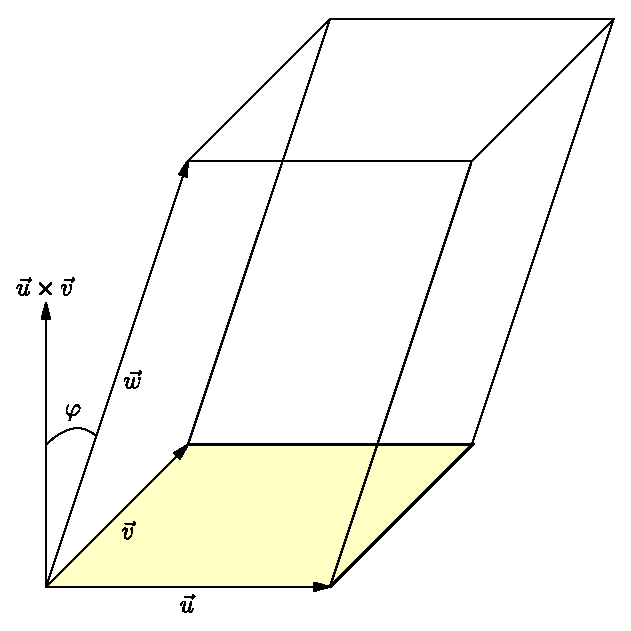
\includegraphics{./cap_algvet/pics/volume_determinante}
   \caption{Representação do paralelepípedo formado por três vetores.}\label{fig:volume_determinante}   
  \end{center}\end{figure}
O triplo produto escalar pode, portanto, ser calculado pelo determinante da matriz formada pelas componentes dos três vetores envolvidos. A expressão do triplo produto escalar como o determinante dos três vetores poderia ter sido mais rapidamente obtido usando (\ref{detprodvec}) o determinante formal que, alternativamente, define o produto vetorial:
\begin{equation}
\vct{u}\cdot (\vct{v}\times \vct{w})
=\left(u_1\vct{i}+u_2\vct{j}+u_3\vct{k}\right)\cdot\left|\begin{array}{ccc}
\vct{i}&\vct{j}&\vct{k}\\
v_1 & v_2 & v_3\\
w_1 & w_2 & w_3\\
\end{array}
\right|=\left|\begin{array}{ccc}
	  u_1&u_2&u_3\\
	  v_1&v_2&v_3\\
	  w_1&w_2&w_3
       \end{array}
 \right|
\end{equation}



Sabemos que quando permutamos duas linhas de uma matriz, seu determinante muda de sinal, pelo que podemos obter as seguintes relações:
\begin{eqnarray*}
\vct{u}\cdot\left(\vct{v}\times\vct{w}\right)&=&-\vct{v}\cdot\left(\vct{u}\times\vct{w}\right)=\vct{v}\cdot\left(\vct{w}\times\vct{u}\right)\\
&=&-\vct{w}\cdot\left(\vct{v}\times\vct{u}\right)=\vct{w}\cdot\left(\vct{u}\times\vct{v}\right)=-\vct{u}\cdot\left(\vct{w}\times\vct{v}\right)  
\end{eqnarray*}
Extraindo apenas os termos de ordem ímpar temos:
\begin{equation}\label{triploprodutoescalar} \vct{u}\cdot\left(\vct{v}\times\vct{w}\right)=\vct{v}\cdot\left(\vct{w}\times\vct{u}\right)=\vct{w}\cdot\left(\vct{u}\times\vct{v}\right)
\end{equation}
\begin{obs} Um caso particular interessante é quando escolhemos $\vct{w}=\vct{u}\times\vct{v}$ e obtemos:
\begin{equation*} 
\det\left(\vct{u},\vct{v},\vct{u}\times\vct{v}\right)=\left(\vct{u}\times\vct{v}\right)\cdot\left(\vct{u}\times\vct{v}\right)=\|\vct{u}\times\vct{v}\|^2.
\end{equation*}
Assim, retornamos à expressão (\ref{propprodvecorient}).
\end{obs}

Podemos igualmente definir o triplo produto vetorial como o produto vetorial de um vetor pelo produto vetorial de outros dois vetores, isto é:
$$\vct{u}\times \left(\vct{v}\times\vct{w}\right). $$
Observe cuidadosamente que o produto vetorial não é associativo, isto é, pode acontecer $\vct{u}\times \left(\vct{v}\times\vct{w}\right)\neq \left(\vct{u}\times \vct{v}\right)\times\vct{w} $ (ver problema \ref{prodvecnaoassoc}), portanto, a ordem dos vetores é relevante.2
Podemos mostrar que o triplo produto vetorial pode ser expresso como:
\begin{equation*} 
\vct{u}\times\left(\vct{v}\times\vct{w}\right)=\left(\vct{u}\cdot\vct{w}\right)\vct{v}-\left(\vct{u}\cdot\vct{v}\right)\vct{w}
\end{equation*}
Para verificar esta identidade, retornamos ao produto vetorial entre $\vct{v}$ e $\vct{w}$ em coordenadas cartesianas e o escrevemos como a diferença entre dois vetores:
\begin{eqnarray*} \vec{v}\times\vec{w}&=&\left(v_2w_3-v_3w_2\right)\vct{i}+\left(v_3w_1-v_1w_3\right)\vct{j}+\left(v_1w_2-v_2w_1\right)\vct{k}\\
&=& \underbrace{\left(v_2w_3\vct{i}+v_3w_1\vct{j}+v_1w_2\vct{k}\right)}_{\vct{p_1}} -\underbrace{\left(v_3w_2\vct{i}+v_1w_3\vct{j}+v_2w_1\vct{k}\right)}_{\vct{p_2}}=\vct{p_1}-\vct{p_2}.
\end{eqnarray*}


\begin{eqnarray*}
\vct{u}\times\vct{p_1}&=& \left(u_1\vct{i}+u_2\vct{j}+u_3\vct{k}\right)\times \left(v_2w_3\vct{i}+v_3w_1\vct{j}+v_1w_2\vct{k}\right)\\
&=&\left(u_2v_1w_2-u_3v_3w_1\right)\vct{i}+\left(u_3v_2w_3-u_1v_1w_2\right)\vct{j}+\left(u_1v_3w_1-u_2v_2w_3\right)\vct{k}\\
&=&\left(u_2v_1w_2\vct{i}+u_3v_2w_3\vct{j}+u_1v_3w_1\vct{k}\right)-\left(u_3v_3w_1\vct{i}+u_1v_1w_2\vct{j}+u_2v_2w_3\right)\vct{k}
\end{eqnarray*}

\begin{eqnarray*}
\vct{u}\times\vct{p_2}&=& \left(u_1\vct{i}+u_2\vct{j}+u_3\vct{k}\right)\times \left(v_3w_2\vct{i}+v_1w_3\vct{j}+v_2w_1\vct{k}\right)\\
&=&\left(u_2v_2w_1-u_3v_1w_3\right)\vct{i}+\left(u_3v_3w_2-u_1v_2w_1\right)\vct{j}+\left(u_1v_3w_1-u_2v_3w_2\right)\vct{k}\\
&=&\left(u_2v_2w_1\vct{i}+u_3v_3w_2\vct{j}+u_1v_3w_1\vct{k}\right)
-\left(u_3v_1w_3\vct{i}+u_1v_2w_1\vct{j}u_2v_3w_2\vct{k}\right)
\end{eqnarray*}

Subtraíndo temos:
\begin{eqnarray*}
\vct{u}\times\left(\vct{p_1}-\vct{p_2}\right)&=&    \left[\left(u_2w_2+u_3w_3\right)v_1\vct{i}+\left(u_1w_1+u_3w_3\right)v_2\vct{j}+\left(u_1w_1+u_2w_2\right)v_3\vct{k}\right]\\
&-&
\left[\left(u_2v_2+u_3v_3\right)w_1\vct{i}+\left(u_1v_1+u_3v_3\right)w_2\vct{j}+\left(u_1v_1+u_2v_2\right)w_3\vct{k}\right]
\end{eqnarray*}
Agora, somamos $u_1v_1w_1$ à primeira coordenada de cada um dos dois termos da subtração; somamos $u_2v_2w_2$  à segunda coordenada de cada um dos dois termos da subtração e somamos $u_3v_3w_3$ à terceira coordenada de cada um dos dois termos da subtração para obter:
% \begin{eqnarray*}
% \vct{u}\times\left(\vct{p_1}-\vct{p_2}\right)&=&    \left[\left(u_1w_1+u_2w_2+u_3w_3\right)v_1\vct{i}+\left(u_1w_1+u_2w_2+u_3w_3\right)v_2\vct{j}+\left(u_1w_1+u_2w_2+u_3w_3\right)v_3\vct{k}\right]\\
% &-&
% \left[\left(u_1v_1+u_2v_2+u_3v_3\right)w_1\vct{i}+\left(u_1v_1+u_2v_2+u_3v_3\right)w_2\vct{j}+\left(u_1v_1+u_2v_2+u_3v_3\right)w_3\vct{k}\right]\\
% &=&(\vct{u}\cdot\vct{w})\vct{v}-(\vct{u}\cdot\vct{v})\vct{w}.
% \end{eqnarray*}
 \begin{eqnarray*}
 \vct{u}\times\left(\vct{p_1}-\vct{p_2}\right)&=&    \left[\left(\vct{u}\cdot\vct{w}\right)v_1\vct{i}+\left(\vct{u}\cdot\vct{w}\right)v_2\vct{j}+\left(\vct{u}\cdot\vct{w}\right)v_3\vct{k}\right]\\
 &-&
 \left[\left(\vct{u}\cdot\vct{v}\right)w_1\vct{i}+\left(\vct{u}\cdot\vct{v}\right)w_2\vct{j}+\left(\vct{u}\cdot\vct{v}\right)w_3\vct{k}\right]\\
 &=&(\vct{u}\cdot\vct{w})\vct{v}-(\vct{u}\cdot\vct{v})\vct{w}.
 \end{eqnarray*}
Lembrando que $\vct{p_1}-\vct{p_2}=\vct{v}\times\vct{w}$, obtemos:
\begin{eqnarray*}
\vct{u}\times\left(\vct{p_1}-\vct{p_2}\right)&=& 
\vct{u}\times\left(\vct{v}\times\vct{w}\right)=(\vct{u}\cdot\vct{w})\vct{v}-(\vct{u}\cdot\vct{v})\vct{w}.
\end{eqnarray*}
O formulário abaixo resume as indentidades que acabamos de demonstrar e lista mais algumas sem demonstração:

\clearpage
\begin{subequations}\label{vectoridendities}
\begin{align}
 \vec{u}\cdot\left(\vec{v}\times\vec{w}\right)&=\vec{v}\cdot\left(\vec{w}\times\vec{u}\right)=\vec{w}\cdot\left(\vec{u}\times\vec{v}\right),&\mytext{Triplo produto escalar}\\ 
 \vec{u}\times\left(\vec{v}\times\vec{w}\right)&=\left(\vec{u}\cdot\vec{w}\right)\vec{v}-\left(\vec{u}\cdot\vec{v}\right)\vec{w},&\mytext{Triplo produto vetorial} \\ 
 \left(\vec{u}\times\vec{v}\right)\times\vec{w}&=\left(\vec{u}\cdot\vec{w}\right)\vec{v}-\left(\vec{v}\cdot\vec{w}\right)\vec{u},&\mytext{Triplo produto vetorial} \\ 
 \left(\vec{u}\times\vec{v}\right)\cdot\left(\vec{w}\times\vec{x}\right)&=\left(\vec{u}\cdot\vec{w}\right)\left(\vec{v}\cdot\vec{x}\right)-\left(\vec{v}\cdot\vec{w}\right)\left(\vec{u}\cdot\vec{x}\right),& \\	 
\left(\vec{u}\cdot\left(\vec{v}\times\vec{w}\right)\right)\vec{x}&=\left(\vec{u}\cdot\vec{x}\right)\left(\vec{v}\times\vec{w}\right)+\left(\vec{v}\cdot\vec{x}\right)\left(\vec{w}\times\vec{u}\right)+\left(\vec{w}\cdot\vec{x}\right)\left(\vec{u}\times\vec{v}\right),& \\
\left(\vec{u}\times\vec{v}\right)\times\left(\vec{w}\times\vec{x}\right)
&=\left(\vec{u}\cdot\left(\vec{v}\times\vec{x}\right)\right)\vec{w}-\left(\vec{u}\cdot\left(\vec{v}\times\vec{w}\right)\right)\vec{x},&\\
\end{align}
\end{subequations}
\newpage


\section{Sistema de coordenadas cilíndricas}

\begin{figure}%[.5\baselineskip]
\begin{center}
   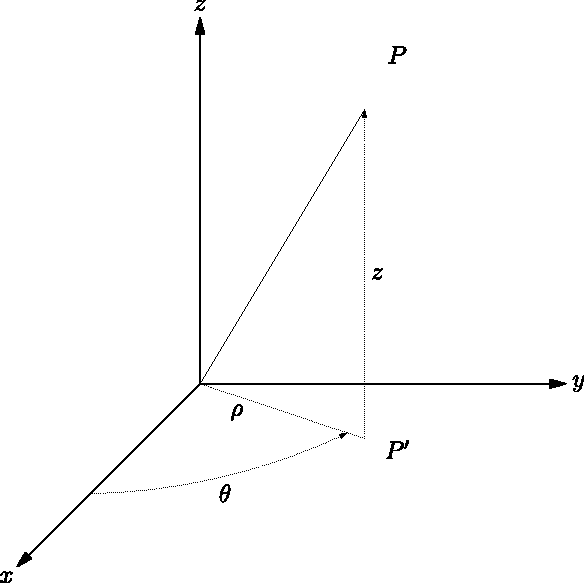
\includegraphics{./cap_algvet/pics/coordenadas_cilindricas}
   \caption{Representação de um ponto de coordenadas cilíndricas.}\label{Coo_cil}   
      \label{fig:coordenadas_cilindricas}
      %\setfloatalignment{b}% forces caption to be bottom-aligned
      \end{center}
  \end{figure}


No sistema de coordenadas cilíndricas, um ponto $P$ é representado pelas coordenadas\index{Sistema de coordenadas cilíndricas} $\rho$, $\theta$ e $z$. A coordenada $z$ é a mesma do sistema de coordenadas retangulares. A coordenada $\rho$ indica a distância entre a origem e a projeção $P'$ de $P$ sob o eixo $xy$. Finalmente $\theta$ é o ângulo entre o semi-eixo $x>0$ e o ponto $P'$. Ver figura \ref{fig:coordenadas_cilindricas}. É fácil ver que
\begin{subequations}\label{xphi}
\begin{eqnarray}
x&=&\rho\cos\theta\\
y&=&\rho\sin\theta
\end{eqnarray}  
\end{subequations}
onde
\begin{equation}
\rho=\sqrt{x^2+y^2}
\end{equation}
A coordenadas $\rho$, $\theta$ e $z$ são comumente denominadas, respectivamente, de ``distância radial'', ``azimute'' e ``altura''. 

As equações (\ref{xphi}) podem ser reescritas como
\begin{subequations}\label{phix}
\begin{eqnarray}
\cos\theta&=&\frac{x}{\rho}=\frac{x}{\sqrt{x^2+y^2}}\\
\sin\theta&=&\frac{y}{\rho}=\frac{y}{\sqrt{x^2+y^2}}
\end{eqnarray}  
\end{subequations}

\begin{exer}\label{rect_cin} Os seguintes pontos são dados em coordenadas cartesianas, encontre suas representações em coordenas cilíndricas:
\begin{itemize}
\item [a)] $\left<1,1,1\right>$
\item [b)] $\left<1,-1,1\right>$
\item [c)] $\left<-1,1,1\right>$
\item [d)] $\left<-1,-1,1\right>$
\end{itemize}
\end{exer}
Resp: $\left(\sqrt{2},\frac{\pi}{4},1\right)$,  $\left(\sqrt{2},\frac{5\pi}{4},1\right)$, $\left(\sqrt{2},\frac{3\pi}{4},1\right)$ e  $\left(\sqrt{2},\frac{7\pi}{4},1\right)$.

\begin{exer} Encontre uma expressão para distância de um ponto à origem em coordenadas cilíndricas
\end{exer}
Resp: $\sqrt{\rho^2+z^2}$
% 



  
 \section{Sistema de coordenadas esféricas}
\begin{figure}%[.5\baselineskip]
\begin{center}
      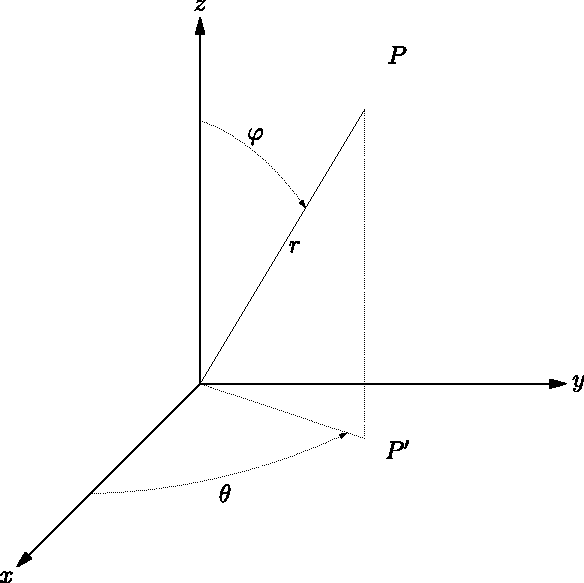
\includegraphics{./cap_algvet/pics/coordenadas_esfericas}
   \caption{Representação de um ponto de coordenadas esféricas.}\label{./cap_algvet/pics/coo_esf}
      \label{fig:coordenadas_esfericas}
        \end{center}\end{figure}

 
 No sistema de coordenadas cilíndricas, um ponto $P$ é representado pelas coordenadas\index{Sistema de coordenadas esféricas} $r$, $\theta$ e $\varphi$. A coordenada $r$ indica a distância do ponto $P$ até a origem, sendo consistente com a definição de módulo de um vetor. A coordenada $\theta$ é o mesmo ângulo do sistema de coordenadas cilíndricas, ou seja,  é o ângulo entre o semi-eixo $x>0$ e o ponto $P'$ (projeção de P no plano xy). O ângulo $\varphi$ é o ângulo entre a reta que liga a origem até o ponto $P$ e o semi-eixo $z>0$.  Ver figura \ref{fig:coordenadas_esfericas}. A relação entre a coordenadas no sistema de coordenadas esféricas e no sistema de coordenadas cilíndricas é dada pelas projeções:
\begin{subequations}
\begin{eqnarray}
z&=&r\cos\varphi\\
\rho&=&r\sin\varphi
\end{eqnarray} 
\end{subequations}
Usando (\ref{xphi}), encontramos a relação entre o sistema de coordenadas esféricas e cartesianas:
\begin{subequations}
\begin{eqnarray}
x&=&r\sin\varphi\cos\theta\\
y&=&r\sin\varphi\sin\theta\\
z&=&r\cos\varphi
\end{eqnarray} 
\end{subequations}
Analogamente, pode-se escrever:
\begin{subequations}
\begin{eqnarray}
r&=&\displaystyle \sqrt{x^2+y^2+z^2}\\
\cos\varphi&=&\displaystyle\frac{z}{r}=\frac{z}{x^2+y^2+z^2}\\
\cos\theta&=&\displaystyle\frac{x}{\rho}=\frac{x}{x^2+y^2}\\
\sin\theta&=&\displaystyle\frac{y}{\rho}=\frac{y}{x^2+y^2}
\end{eqnarray} 
\end{subequations}


\begin{exer}\label{rect_esf} Os seguintes pontos são dados em coordenadas cartesianas, encontre suas representações em coordenas esféricas (ver também excício \ref{rect_cin}):
\begin{itemize}
\item [a)] $\left<1,1,1\right>$
\item [b)] $\left<1,-1,1\right>$
\item [c)] $\left<-1,1,1\right>$
\item [d)] $\left<-1,-1,1\right>$
\end{itemize}
\end{exer}
Resp: $\left(\sqrt{3},\frac{\pi}{4},\theta\right)$,  $\left(\sqrt{3},\frac{5\pi}{4},\theta\right)$, $\left(\sqrt{3},\frac{3\pi}{4},\theta\right)$ e  $\left(\sqrt{3},\frac{7\pi}{4},\theta\right)$, onde $\theta=\cos^{-1}\left(\frac{\sqrt{3}}{3}\right)\approx 0,955.$



\section{Exemplos na física}
Na mecânica, o trabalho de uma força\index{trabalho de uma força} constante atuando sobre um corpo que se move com velocidade constante é dado pelo produto escalar da força pelo deslocamento:
$$W=\vct{F}\cdot \triangle\vct{ r}$$
O torque de uma força em relação a um eixo dado é dado por
$$\vct{\tau}=\vct{r}\times \vct{F}$$
onde $\vct{r}$ é o vetor que liga o ponto onde a força é aplicada e o pondo onde o torque é medido. 

A força $\vct{F}$ que uma campo magnético $\vct{B}$ produz em uma partícula de carga elétrica $q$ em movimento com velocidade $\vct{v}$ é dado pela lei de Lorentz:
$\vct{F}=q\vct{v}\times\vct{B}.$

\section{Notas avançadas}
\subsection{O que é um espaço linear?}
A definição de espaço vetorial dada em (\ref{defel}) é ampla e engloba conceitos bem mais gerais que os espaços euclidianos de dimensão 2 e 3 com os quais o leitor tem maior familiaridade. As funções reais $f:\mathbb{R}\to\mathbb{R}$, por exemplo, formam espaço vetorial onde os escalares são dados pelos números reais. O vetor nulo, neste caso, é a função $f(x)=0$. Este espaço não tem dimensão finita pois os polinômios $P_{n}(x)=x^n$ para $n=0,1,2,3,\ldots$ formam uma família infinita de vetores linearmente independentes (isso é uma consequência do teorema fundamental da álgebra).      

\subsection{Todo espaço linear tem uma base? Axioma da escolha.}
Um problema importante é descobrir se todo espaço linear admite uma base. Este problema é mais complicado do que pode parecer e conduz a uma profunda discussão sobre os próprios fundamentos da matemática. De fato, pode-se mostrar que, o axioma da escolha implica que todo espaço linear tenha uma base. 

O axioma da escolha é um dos axiomas da teoria de conjuntos padrão que tem diversas consequências contraintuitivas e fisicamente inesperadas. Um exemplo das bizarrias produzidas pelo axioma da escolha é o chamado paradoxo de Banach-Tarski: Dada uma esfera no espaço euclidiano de três dimensões, é possível cortá-la em um número finito de pedaços e rearranjar esses pedaços de forma a construir duas esferas idênticas à original. Em outras palavras, o axioma da escolha aplicado ao espaço euclidiano tridimensional traz como consequências a não preservação de ``volume'' frente a translações e rotações. Para definir de forma razoável os conceitos de comprimento, área e volumes, foi necessário o desenvolvimento da teoria da medida no final do Século XIX e início do Século XX. A solução encontrada foi construir uma medida apenas em uma família de subconjuntos chamamos conjuntos mensuráveis.      

Vejamos um exemplo de espaço linear de dimensão: é fácil verificar que o conjunto de todos os polinômios $P(x)=a_0+a_1x+a_2x^2+\ldots a_nx^n$ formam um espaço linear frente às operações usuais de soma e multiplicação por um escalar. A base deste espaço é dada pelos monômios $P_{n}(x)=x^n$ para $n=0,1,2,3,\ldots$ pois cada polinômio pode ser escrito como uma combinação linear \emph{finita} de elementos desse base. No entanto, não é possível mostrar desta forma contrutiva uma base para o espaço das funções reais ou mesmo para as funções reais contínuas. A existência de uma base para estes espaços é um conceito abstrato  não contrutivo.

\subsection{Qual amplo é o conceito de norma?}
Vimos que o conceito de espaço linear é muito mais amplo e útil que parecia. E quanto à norma? Estamos familiariados com a norma euclidiana, mas será que é possível definir outras normas no espaço $\mathbb{R}^n$ de forma a satisfazer as propriedades (\ref{propnorma})? A norma euclidiana em um espaço de dimensão $n$ é dada por
$$\|\vct{x}\|=\left(x_1^2+x_2^2+\ldots x_n^2\right)^{1/2}$$
De fato é possível mostrar que podemos alterar esta expressão para
$$\|\vct{x}\|_p=\left(|x_1|^p+|x_2|^p+\ldots +|x_n|^p\right)^{1/p}$$
com $p\geq 1$ de forma a preservar todas as propriedades da norma.

Mas será que é possível definir uma norma no espaço das funções reais? Esta é uma pergunta complicada, mas podemos simplificar exigindo um pouco mais desse espaço. Por exemplo, vamos considerar o espaço das funções reais contínuas definidas no intervalo $[0,1]$. Neste espaço é possível definir a seguinte norma:
\begin{equation}\label{norma_infinito}\|f(x)\|=\max_{x\in [0,1]}|f(x)|\end{equation}

ou seja, a norma de uma função contínua é dada pelo máximo de seu módulo no intervalo.

No entanto, esta não é a única maneira de definir uma norma neste espaço, outra possibilidade é:
\begin{equation}\label{norma_lp}\|f(x)\|_{p}=\left(\int_0^1|f(x)|^pdx\right)^p\end{equation}
onde $p\geq 1$.

A norma (\ref{norma_lp}) é chamada de norma $L^p$ de uma função e a norma (\ref{norma_infinito}) é chamada de norma do máximo ou norma infinito ou norma $L^{\infty}$. Isso porque
$$\lim_{p\to\infty}\|f(x)\|_{p}=\max_{x\in [0,1]}|f(x)|.$$

Esta normas excem enorme importância na teoria de funções com importantes aplicações no estudo das equações diferenciais. 

\subsection{E o produto escalar?}
Uma operação com as propriedades (\ref{proprodesc}) é um produto escalar. Produtos escalares não aparecem apenas em espaços de duas ou três dimensões: mesmo espaços de dimensão infinita podem possuir um produto escalar. Tomemos como exemplo novamente o espaço das funções contínuas definidas no intervalo $[0,1]$. A seguinte operação possui todas as propriedades de um produto escalar:
$$\left<f,g\right>=\int_0^1f(x)g(x)dx.$$
Observe o leitor que foi usada a notação $\left<,\right>$ para indicar o produto interno. Este produto interno induz a seguinte norma:
$$\|f\|_2=\left(\left<f,f\right>\right)^{1/2}=\left(\int_0^1f(x)^2dx\right)^{1/2}$$
que é o caso particular de (\ref{norma_lp}) quando $p=2$. 
 A desigualdade de Cauchy-Schwarz admite a seguinte forma:
$$\int_0^1f(x)g(x)dx \leq \left(\int_0^1f(x)^2dx\right)^{1/2} \left(\int_0^1g(x)^2dx\right)^{1/2}$$
  %\chapter{Álbegra vetorial}

\chapter{Funções de várias variáveis}

\chapter{Integrais múltiplas}


%%%%%%%%%%%%%%%%%%%%%%%%%%%%%%%%%%%%%%%%
%%%%%%%%%%      Parte 3       %%%%%%%%%%
%%%%%%%%%%%%%%%%%%%%%%%%%%%%%%%%%%%%%%%%

\part{Cálculo em variedades}

\chapter{Curvas e trajetórias}
\chapter{Integral de linha}
\chapter{Superfícies}
\chapter{Teorema da Divergência de Gauss}
\chapter{Teorema de Stokes}
\chapter{Formulação intínseca dos operadores diferenciais}









%%
% The back matter contains appendices, bibliographies, indices, glossaries, etc.







\backmatter

\bibliography{main}
\bibliographystyle{plainnat}


\printindex

\end{document}

